\subsection{Futures}
\begin{frame}[fragile]{without Futures}
\begin{lstlisting}[frame=htrbl]
someCombinator :: [arr a b] -> [arr b c] -> arr [a] [c]
someCombinator fs1 fs2 =
	parEvalN () fs1 >>>	rightRotate >>>	parEvalN () fs2
\end{lstlisting}
\pause
\begin{center}
\includegraphics[scale=0.3]{images/withoutFutures}
\end{center}
\end{frame}
\begin{frame}[fragile]{Future definition}
Since the particular concepts and implementations differ from backend to backend, we define the Future typeclass:
\begin{lstlisting}[frame=htrbl]
class Future fut a conf | a conf -> fut where
    put :: (Arrow arr) => conf -> arr a (fut a)
    get :: (Arrow arr) => conf -> arr (fut a) a
\end{lstlisting}
\end{frame}
\begin{frame}[fragile]{Future implementation (Eden)}
\begin{lstlisting}[frame=htrbl]
data RemoteData a = RD { rd :: RD a }

put' :: (Arrow arr) => arr a (BasicFuture a)
put' = arr BF

get' :: (Arrow arr) => arr (BasicFuture a) a
get' = arr (\(~(BF a)) -> a)

instance NFData (RemoteData a) where
    rnf = rnf . rd
instance Trans (RemoteData a)

instance (Trans a) => Future RemoteData a Conf where
    put _ = put'
    get _ = get'
\end{lstlisting}
\end{frame}
\begin{frame}[fragile]{with Futures}
\begin{lstlisting}[frame=htrbl]
someCombinator :: [arr a b] -> [arr b c] -> arr [a] [c]
someCombinator fs1 fs2 =
	parEvalN () (map (>>> put ()) fs1) >>>
	rightRotate >>>
	parEvalN () (map (get () >>>) fs2)
\end{lstlisting}
\pause
\begin{center}
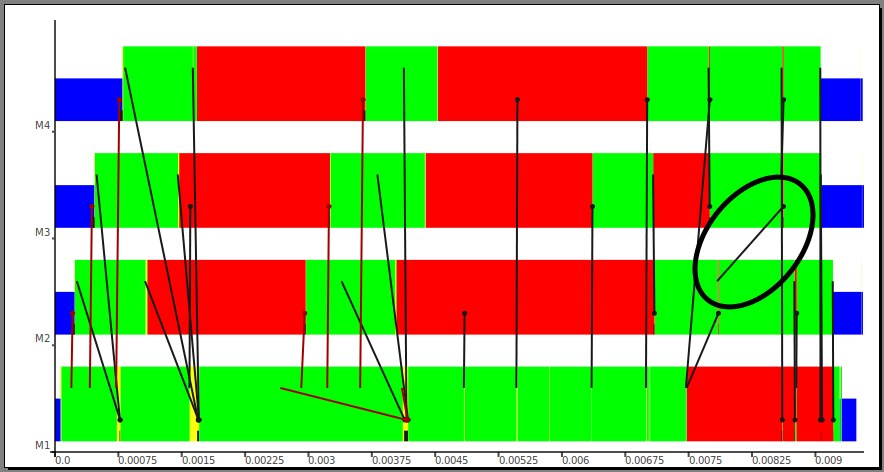
\includegraphics[scale=0.35]{images/withFutures}
\end{center}
\end{frame}